\chapter{Métodos Numéricos \label{cap:num}}
En este capítulo se presentan los métodos numéricos fundamentales utilizados en el desarrollo de esta tesis. Dado que muchos sistemas fotónicos carecen de soluciones analíticas exactas, los enfoques numéricos resultan esenciales para modelar su comportamiento electromagnético. Estos métodos permiten aproximar soluciones con precisión controlada, incluso en geometrías donde no existe alguna simetría a explotar.

El punto de partida lo constituyen las ecuaciones (\ref{eqn:helmholz}) y (\ref{eqn:helmholzH}), que describen la propagación de campos electromagnéticos en medios dieléctricos. Cuando se aplica la aproximación de guiaje débil los términos del lado derecho de ambas ecuaciones pueden despreciarse. Esta simplificación elimina los efectos cruzados entre componentes de campo, reduciendo el sistema a ecuaciones escalares de tipo Helmholtz:
\begin{equation}
\left[\nabla^2 + k_0^2 n^2(\textbf{r})\right]\Psi(\textbf{r}) = 0, \label{eqn:helmholtznum}
\end{equation}
donde la ecuación (\ref{eqn:helmholtznum}) no solo sirve como marco teórico, sino también como base para los algoritmos desarrollados en los siguientes capítulos. Su versatilidad permite adaptar diferentes esquemas numéricos según las simetrías del problema, como se detallará en las secciones posteriores.
\section{Expansión en Modos Normales \label{cap:eme}}
Este método numérico es útil cuando los sistemas fotónicos en estudio son invariantes en la dirección de propagación $z$. Esto es, $n(\textbf{r})\equiv n(x,y)$. La soluciones de la ecuación (\ref{eqn:helmholtznum}) se pueden expandir en ondas planas con perfiles transversales: $\Psi(\textbf{r}) = \Psi(x,y) \exp({i\beta z})$. Con ésto, cada modo transversal $\nu$ debe cumplir la siguiente ecuación a resolver numéricamente:
\begin{equation}
	\left[\nabla_\perp^2 + k_0^2 n^2(x,y)\right]\Psi_\nu(x,y) = \beta_\nu^2\Psi_\nu(x,y) \ , \quad\text{ con } \nabla_\perp^2 \equiv \frac{\partial^2}{\partial x^2} + \frac{\partial^2}{\partial y^2} \ .
	\label{eqn:eme}
\end{equation}
Y el campo total propagado es una combinación lineal de los modos $\Psi_\nu$: 
\begin{equation}
	\Psi(\textbf{r}) = \sum_\nu a_\nu \Psi_\nu(x,y) e^{i\beta_\nu z}, \quad\text{ con } a_\nu \propto \Psi_\nu(x,y) \cdot \Psi(x, y, z=0). \label{eqn:emedin}
\end{equation}
En vez de integrar directamente la ecuación de valores propios (\ref{eqn:eme}), la estrategia será discretizar el espacio y aproximar al operador laplaciano transversal $\nabla_\perp^2$ como una matriz, pues $$\frac{\partial^2 \Psi(x,y)}{\partial x^2} \sim \frac{\Psi[i+1,j]-2\Psi[i,j]+\Psi[i-1,j]}{\Delta x ^2}  \ .
$$
$\nabla^2_\perp \sim \hat{D}_{xx} \otimes I_y + I_x \otimes \hat{D}_{yy}$
La matriz es nula en las posiciones no diagonales más allá de un espacio (\textit{sparse-like}), por lo que es posible optimizar el proceso de cómputo al utilizar la librería de Python \href{https://docs.scipy.org/doc/scipy/reference/sparse.linalg.html}{\color{magenta}\texttt{scipy.sparse.linalg}}, especialmente diseñada para el álgebra lineal de matrices de escasos elementos. El anexo \ref{sec:codigohelmholtz} contiene una implementación de este algoritmo en Python bajo \href{https://www.gnu.org/licenses/gpl-3.0.html}{\color{magenta}licencia GNU GPL v3}.

En la Figura \ref{fig:emenumerror} se valida el método numérico mediante comparación con las soluciones analíticas obtenidas en la subsección \ref{cap:solslabTETM}. La complejidad del problema es del orden $O(N^2)$ debido a la construcción de las matrices de $N\times N$, lo que se refleja en la dependencia del tiempo de ejecución en función del paso $\Delta x \equiv \frac{L}{N-1}$.


\begin{figure}[H]
	\centering
	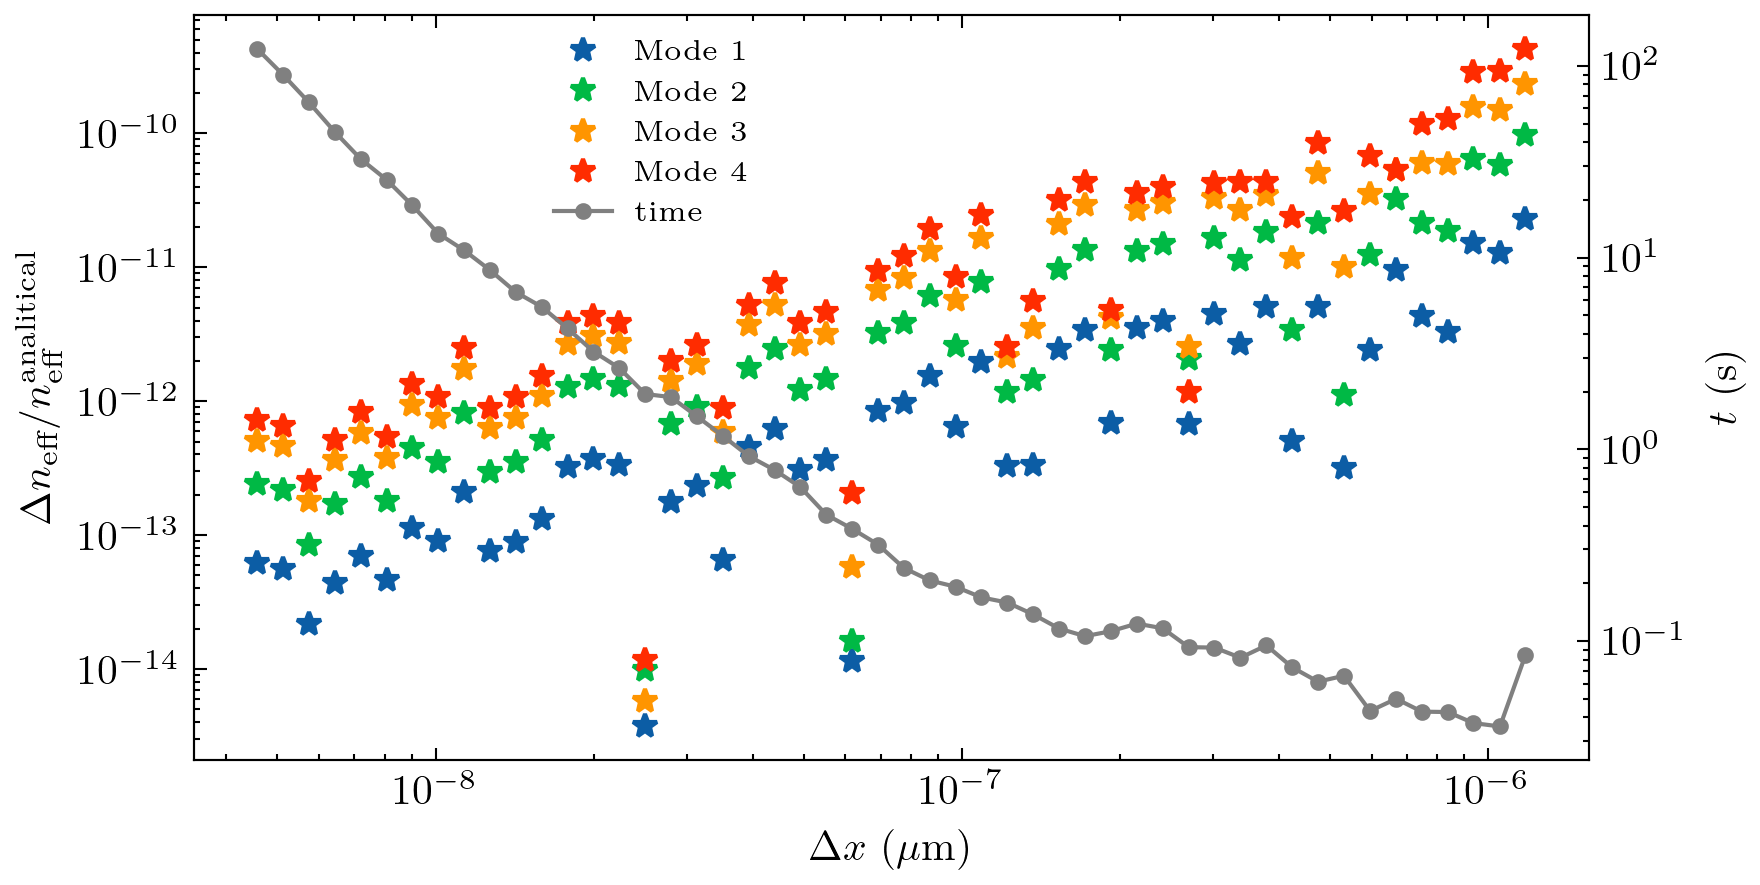
\includegraphics[width=\linewidth]{media/numerical_slab}
	\caption[Error relativo y tiempo de ejecución.]{Error relativo y tiempo de ejecución de las soluciones numéricas a la ecuación (\ref{eqn:eme}) con respecto a las soluciones analíticas, en función del paso $\Delta x$. \label{fig:emenumerror}}
\end{figure}
\section{Método de Propagación de Haces} 
Otra forma de abordar la integración numérica de la ecuación (\ref{eqn:helmholtznum}) consiste en separar el campo en su envolvente lenta y una fase rápidamente oscilante, considerando que en el rango visible el orden de magnitud es, $k_0 \sim 10 ^{5} \text{ cm}^{-1}$: $\Psi(\textbf{r}) = \phi(x,y,z)\exp(ik_0 n_0 z)$. Luego de reemplazar en la ecuación (\ref{eqn:helmholtznum}) se obtiene la ecuación óptica de Schrödinger \citep{paraxialschrodinger}:
\begin{equation}
	-2ik_0 n_0\frac{\partial }{\partial z}\phi(x,y, z) =  \left[\nabla_\perp^2 + k_0^2 (n^2(\textbf{r})-n_0^2)\right]\phi(x,y, z), \label{eqn:bpmescalar}
\end{equation} 
donde se ha utilizado la aproximación paraxial $\left| \frac{\partial^2 \phi}{\partial z^2} \right| \ll 2 k_0 n_0\left| \frac{\partial \phi}{\partial z} \right|$. Los algoritmos que resuelven la ecuación (\ref{eqn:bpmescalar}) son conocidos como Métodos de Propagación de Haces o \textit{Beam Propagation Methods} (BPM) escalares, utilizados ampliamente en esta área de investigación \cite{bics, interorbital, OAMCaging, vortex, bpm}. Fuera de la aproximación de guiaje débil, los efectos de polarización cruzada son más relevantes y se hace necesaria una descripción vectorial del problema.
\subsection{Implementación mediante transformada de Fourier (FFTBPM)}
La ecuación (\ref{eqn:bpmescalar}) se puede escribir en términos de operadores lineales como \citep{bpm}: 
\begin{equation}
	\frac{\partial \phi}{\partial z}  = \left(\hat{A} + \hat{B}\right)\phi, \text{ con } \hat{A} \equiv i\frac{\nabla^2_\perp}{2k_0n_0}\text{ y } \hat{B} \equiv i\frac{k_0}{2n_0}\left[n^2(\textbf{r})-n_0^2\right]. \label{eqn:bpmop}
\end{equation}
La solución formal a la ecuación (\ref{eqn:bpmop}) es $\phi(\textbf{r}) = \exp\left[\left(\hat{A} + \hat{B}\right)(z-z_0)\right]\phi(x, y, z_0)$. Es conveniente trabajar con el operador \( \hat{A} \) en el espacio de Fourier y con el operador \( \hat{B} \) en el espacio directo. Esto se debe a que \( \hat{A} \) contiene derivadas espaciales —en particular, el operador laplaciano transversal \( \nabla^2_\perp \)— las cuales se convierten en multiplicaciones simples al aplicar la transformada de Fourier. De esta forma, la operación \( \hat{A} \phi \) se vuelve computacionalmente eficiente al transformarla en el dominio de los vectores de onda \( \textbf{k}_\perp \), donde actúa como un operador diagonal. Por otro lado, \( \hat{B} \) depende del perfil espacial del índice de refracción \( n(\textbf{r}) \), el cual está definido localmente en el espacio real. Evaluar este término en Fourier implicaría una convolución, lo cual es innecesariamente costoso y menos intuitivo. Por este motivo, se mantiene en el espacio directo. 

Dado que $\hat{A}$ y $\hat{B}$ no conmutan en general, se puede expandir el operador exponencial a orden $O(\Delta z ^3)$ como $\exp\left[\left(\hat{A} + \hat{B}\right)\Delta z \right] \approx \exp\left(\frac{\hat{A}\Delta z}{2} \right)\exp\left(\hat{B}\Delta z \right)\exp\left(\frac{\hat{A}\Delta z}{2} \right) + O(\Delta z ^3)$.

El algoritmo a implementar es el siguiente: \begin{enumerate}
	\item   Se comienza con un perfil $\phi(x, y, z_0)$
\item   Se actúa en el espacio de Fourier transformando el perfil y multiplicado por la fase asociada a $\hat{A}$: $\exp\left(\frac{ik^2\Delta z}{4k_0 n_0}\right)\mathcal{F}(\phi(z_0))$, donde $k=\sqrt{k_x^2 + k_y^2}$ son las frecuencias de Fourier.
\item   Se aplica transformada de Fourier inversa y se multiplica por la fase asociada a $\hat{B}$: 

$\exp\left[\frac{i\Delta z k_0^2(n^2-n_0^2)}{2 k_0n_0}\right]\mathcal{F}^{-1}\left(\exp\left(\frac{ik^2 \Delta z}{4k_0 n_0}\right)\mathcal{F}(\phi(z_0))\right)$
\item  Se regresa al espacio de Fourier y se multiplica por la fase asociada a $\hat{A}$:
 
$\exp\left(\frac{ik^2\Delta z}{4k_0 n_0}\right)\mathcal{F}\left\{\exp\left[\frac{ik_0^2(n^2-n_0^2)}{2 k_0n_0}\Delta z \right]\mathcal{F}^{-1}\left[\exp\left(\frac{ik^2\Delta z}{4k_0 n_0}\right)\mathcal{F}(\phi(z_0))\right]\right\}$
\item Se vuelve al espacio real, habiendo avanzado un paso $\Delta z$:

$\phi(z_0+\Delta z)=\mathcal{F}^{-1}\left\{\exp\left(\frac{ik^2\Delta z}{4k_0 n_0}\right)\mathcal{F}\left\{\exp\left[\frac{i k_0^2(n^2-n_0^2)}{2 k_0n_0}\Delta z\right]\mathcal{F}^{-1}\left[\exp\left(\frac{ik^2\Delta z}{4k_0 n_0}\right)\mathcal{F}(\phi(z_0))\right]\right\} \right\}$

\item Se itera hasta llegar a la distancia de propagación $z$ deseada.
\end{enumerate} En la Figura \ref{fig:num-exp-comp} se comparan los resultados experimentales con las simulaciones numéricas obtenidas mediante BPM. Los perfiles de intensidad normalizados muestran un acuerdo cualitativo notable, particularmente en la distribución espacial de los lóbulos principales.
\begin{figure}[H]
\centering
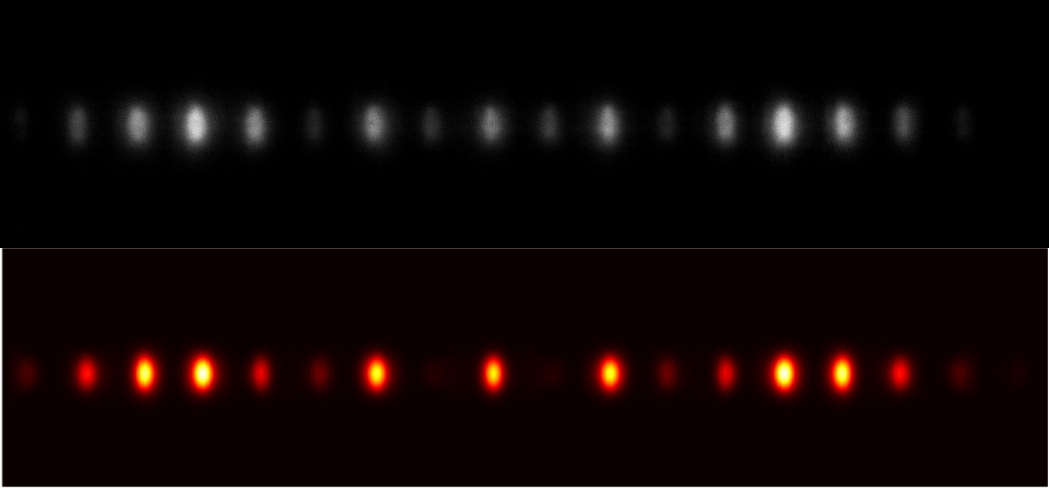
\includegraphics[width=\linewidth]{media/num_exp_comparison.png}
\caption[Excitación del sitio central de una red unidimensional.]{ Excitación del sitio central de una red unidimensional.
\textbf{Arriba:} Medición experimental a $\lambda$ = 730 nm.
\textbf{Abajo:} Simulación numérica realizada con BPM.
\label{fig:num-exp-comp}} \end{figure} Este nivel de concordancia cualitativa valida la aproximación de guiado débil empleada en la ecuación (\ref{eqn:helmholtznum}), así como la aproximación paraxial, y refuerza la confiabilidad del método numérico para el diseño de dispositivos fotónicos con geometrías análogas.
\section{Desde la Teoría de Modos Acoplados \label{cap:CMT}}
La simulación numérica de las ecuaciones (\ref{eqn:non-ortho-CMT-eqs}) representa la formulación más compacta posible, dado que la matriz de acoplamientos $\hat{C} \equiv \hat{P}^{-1}\hat{H}$ codifica todas las propiedades de la red que se desean estudiar de manera semiempírica. En este sentido, la diagonalización de $\hat{C}$ constituye una herramienta numérica valiosa para analizar el comportamiento de redes fotónicas ante variaciones de parámetros como la dimerización (definida como la razón entre dos constantes de acoplamiento) o el desintonizado (la diferencia entre las constantes de propagación de modos distintos). 
Además, este enfoque permite explorar incluso sistemas ``no físicos'', gracias a los grados de libertad disponibles en los elementos de $\hat{C}$: por ejemplo, casos en los que el acoplamiento a segundos vecinos sea mayor que a primeros vecinos, o sistemas con acoplamientos complejos.

En la aproximación de guiaje débil se pueden despreciar las componentes longitudinales del campo eléctrico:
\[ \nabla \cdot (n^2 \textbf{E}) \overset{\nabla n^2 \sim 0}{\sim} n^2 \nabla \cdot \textbf{E} = 0,\]
donde el orden de magnitud de la componente longitudinal del campo es $|E_z| \sim |\nabla_\perp \cdot \textbf{E}_\perp|/\beta$. Así, los modos estudiados son cuasi-transversales, y la matriz $\hat{P}$ se reduce a:
\begin{equation}
    P_{ij} \sim \frac{k_z^i + k_z^j}{4\omega\mu_0} \iint \left(\textbf{e}_i^\perp\right)^* \cdot \textbf{e}_j^\perp dxdy.
    \label{eqn:CMTnum}
\end{equation}
La ecuación (\ref{eqn:CMTnum}), que cuantifica el solapamiento entre modos, junto con la ecuación (\ref{eqn:hij}) que describe los elementos de matriz del operador Hamiltoniano, constituyen herramientas fundamentales para el análisis comparativo entre el método de Expansión en Modos Normales (EME) y la Teoría de Modos Acoplados (CMT). Esta comparación se realiza a través de un estudio sistemático del espectro de autovalores de la matriz de acoplamientos $\hat{C}$, el cual contiene información esencial sobre las constantes de propagación efectivas del sistema. 

La Figura \ref{fig:EMECMT} presenta un análisis cuantitativo de esta comparación, mostrando la evolución de los autovalores para un acoplador fotónico dieléctrico en función de la distancia de separación entre guías. Se observa que ambos métodos convergen asintóticamente para distancias mayores a $d > 20\,\mu$m, donde la aproximación de campo débil de CMT resulta válida. Sin embargo, en el régimen de acoplamiento fuerte ($d < 13\,\mu$m), las discrepancias comienzan a hacerse notar.

Más allá del análisis espectral, la validez de los autoestados calculados puede verificarse indirectamente mediante la ecuación (\ref{eqn:emedin}), que relaciona la evolución del campo con la proyección sobre los modos propios del sistema y comparando cualitativamente los perfiles dinámicos obtenidos con los resultados experimentales y numéricos mostrados en la Figura \ref{fig:num-exp-comp}. Este análisis (ver Figura \ref{fig:1darraycmt}) permite establecer los límites de aplicabilidad de cada método numérico: mientras que EME proporciona resultados precisos en todo el rango de parámetros a costa de mayor complejidad computacional, CMT ofrece una alternativa eficiente para sistemas débilmente acoplados donde la aproximación de modos localizados sigue siendo válida.
\begin{figure}[h]
    \centering
    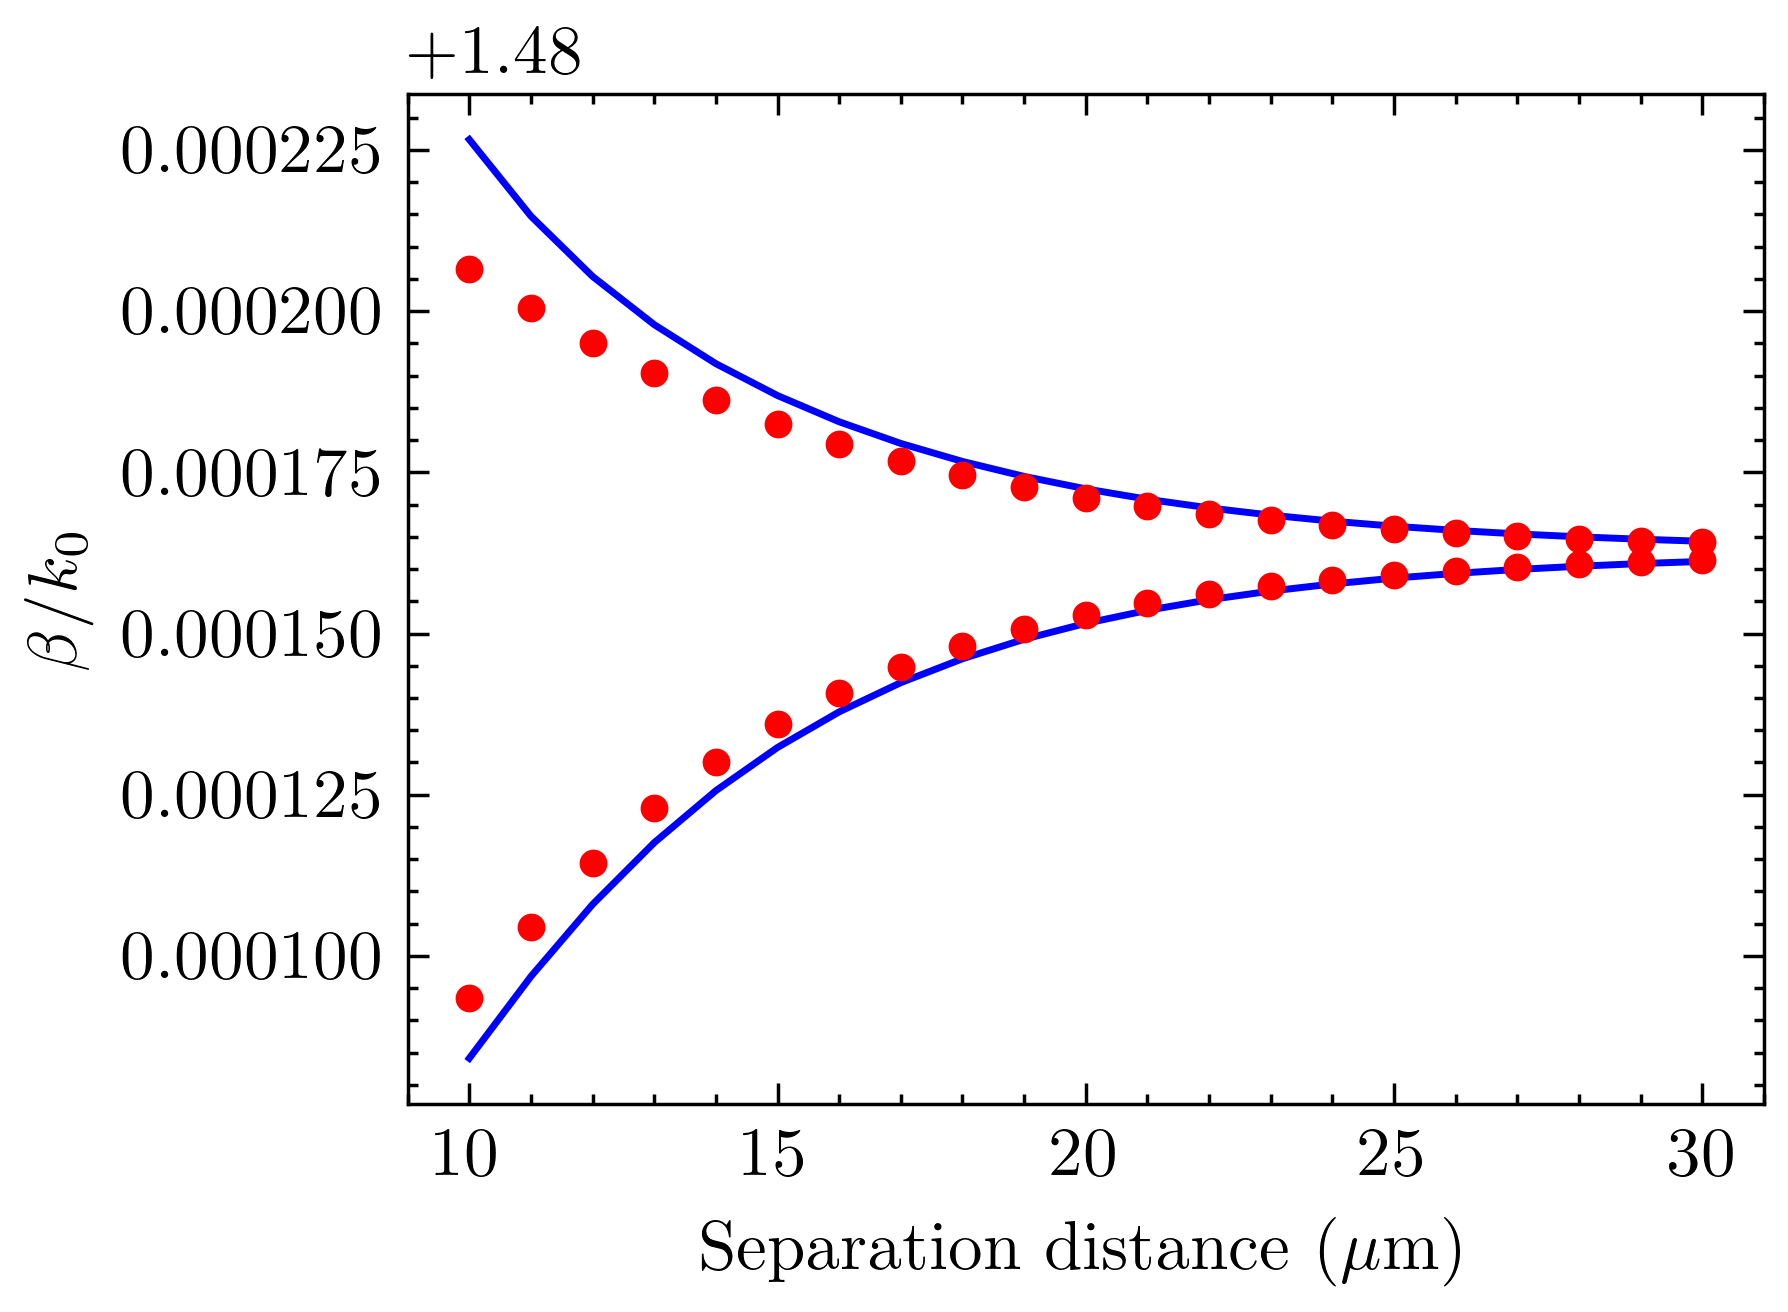
\includegraphics[width=0.8\linewidth]{codigo/dimol/coupler.png}
    \caption[Comparación entre EME y CMT.]{Comparación de los autovalores obtenidos con el método de Expansión en Modos Normales (EME) y con la Teoría de Modos Acoplados (CMT). Se observa mayor divergencia cuando la distancia entre guías es pequeña. Parámetros utilizados: $n_0=1.48$, $\Delta n = 4\times10^{-4}$, $\lambda = 730$ nm y $a = 3\,\mu$m.}
    \label{fig:EMECMT}
\end{figure}
\begin{figure}[h]
	\centering
	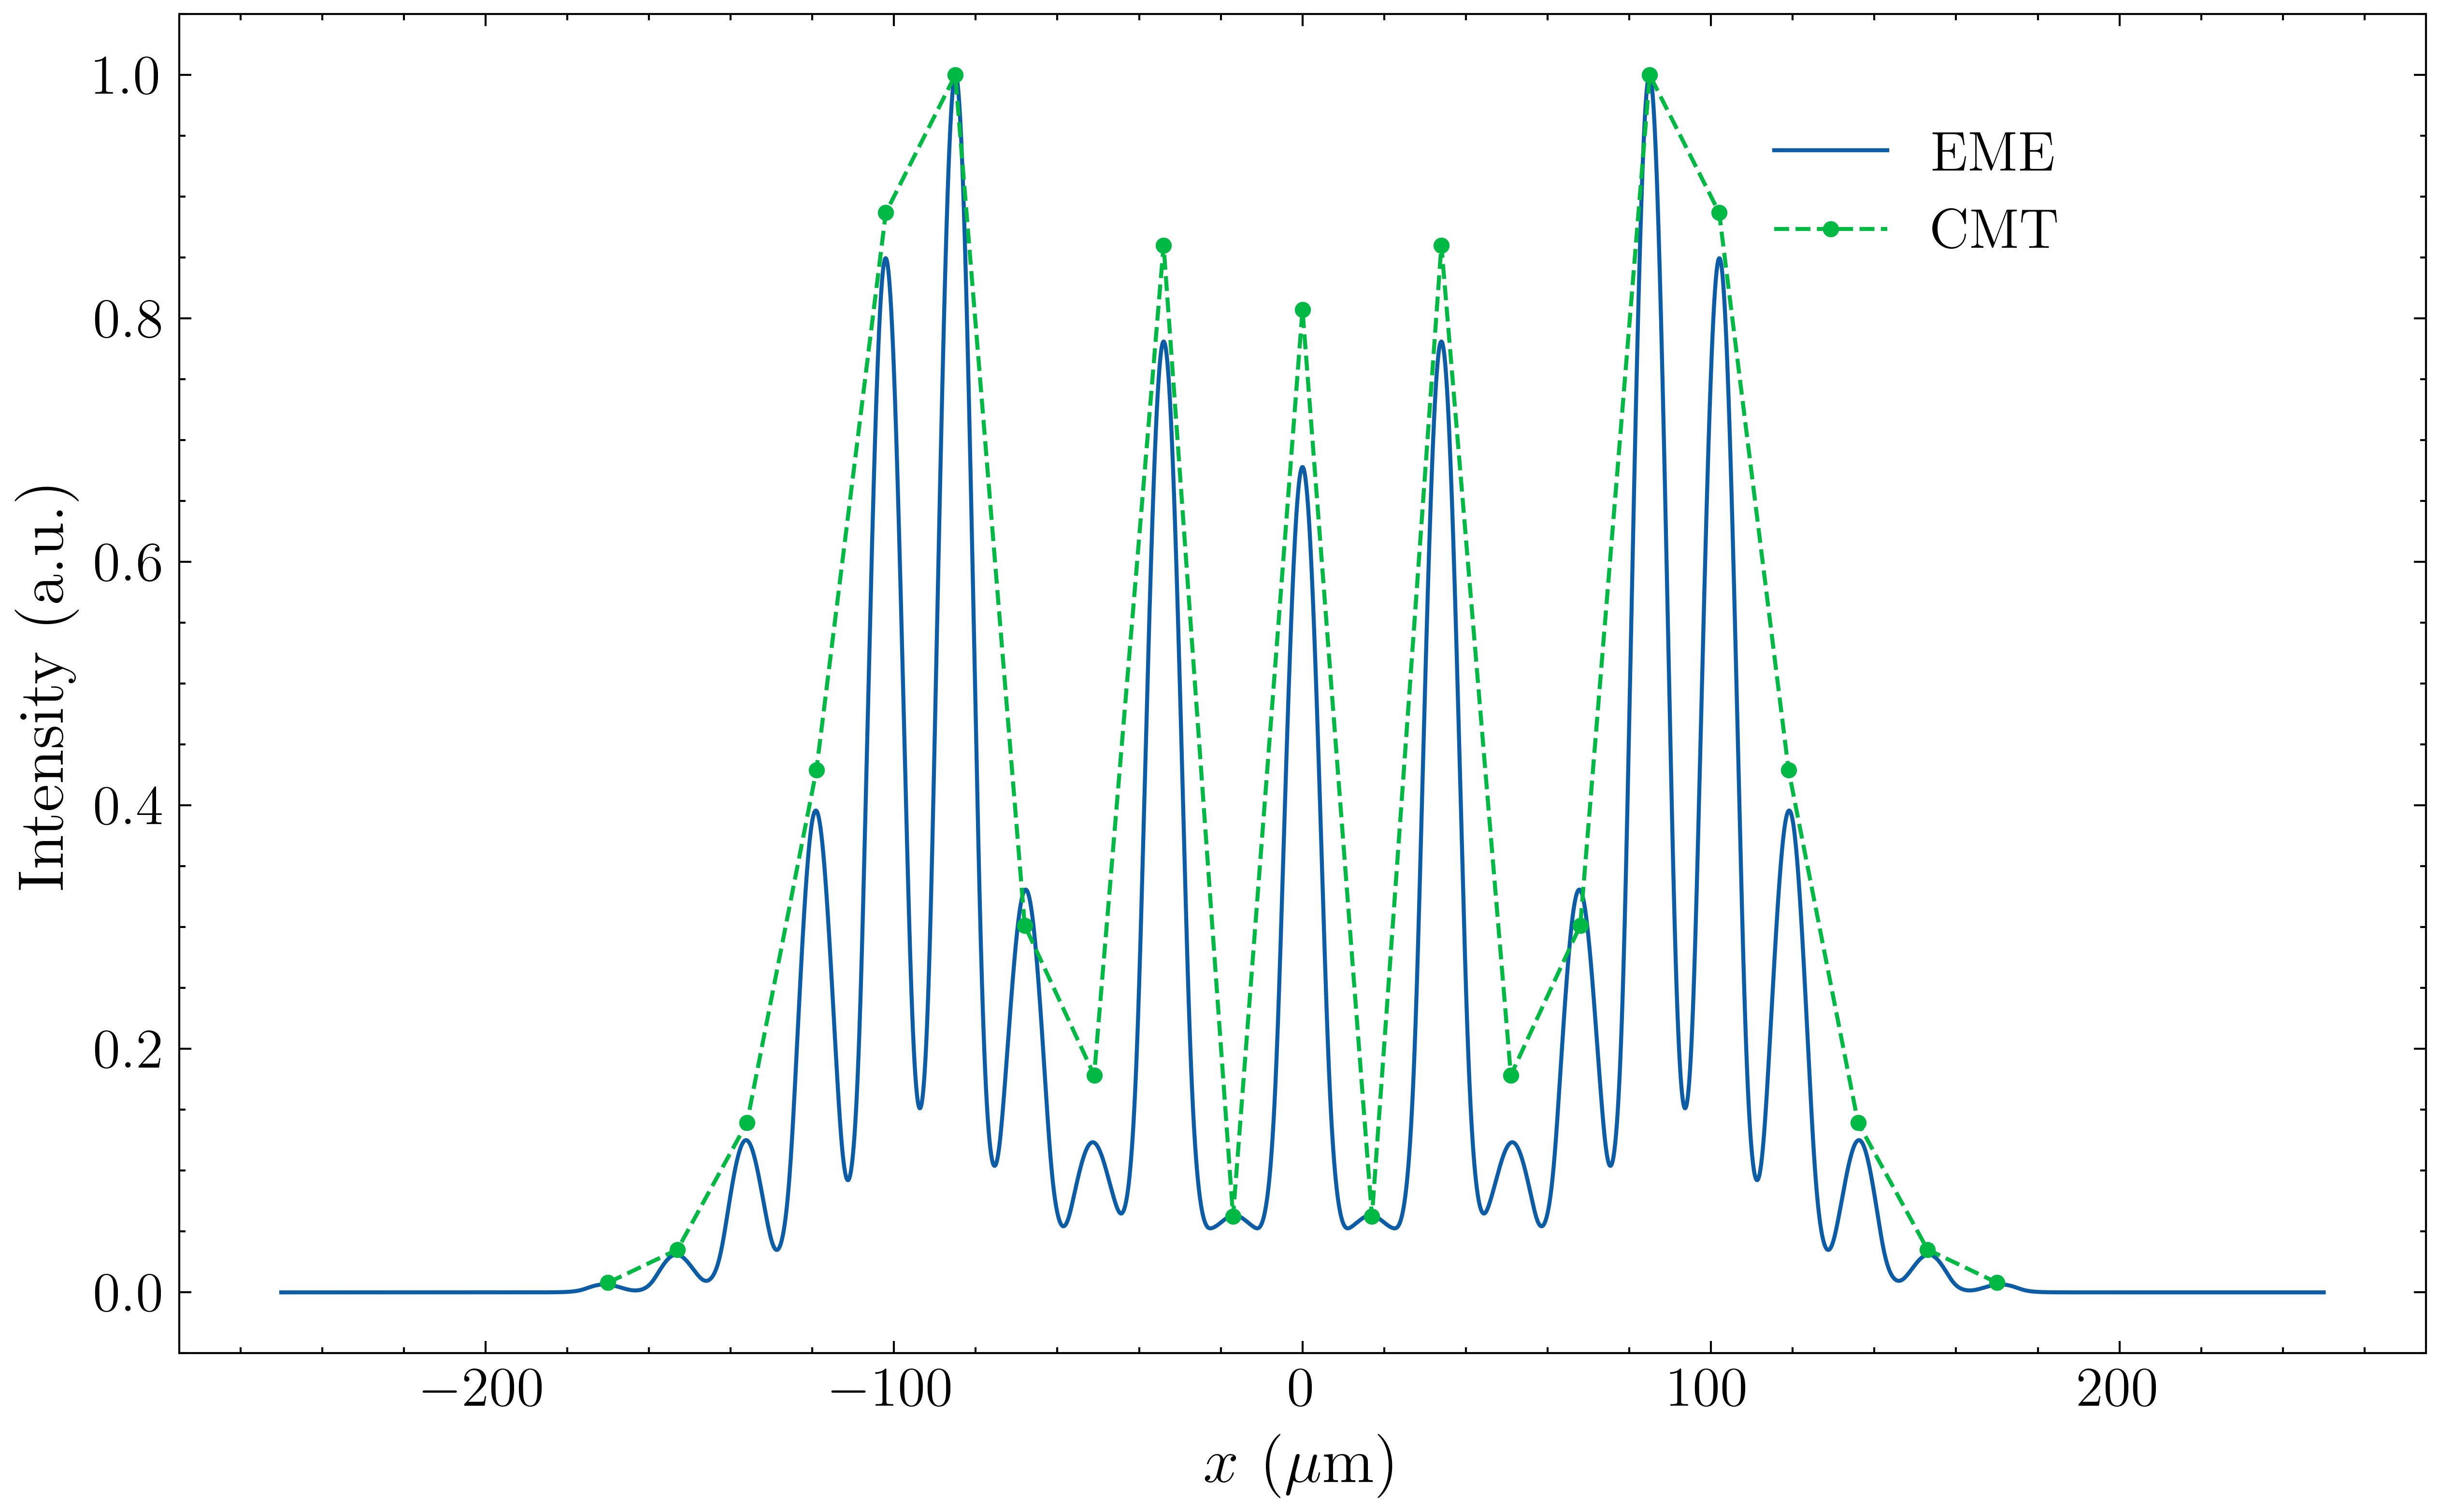
\includegraphics[width=0.8\linewidth]{codigo/1darraycmt/1darraycmt.png}
	\caption[Dinámica con EME y CMT.]{Perfil dinámico de un arreglo unidimensional de 21 guías simulado con CMT y con EME. Los resultados son similares a los de la Figura \ref{fig:num-exp-comp}.}
	\label{fig:1darraycmt}
\end{figure}
